% Standalone source of the massive three-vertex chain of the first application
% example (Sec. 5), redrawn faithfully from the original three_vertex_tree figure:
% three black vertices (the + contour branch) on a horizontal axis, external legs
% drawn as fans above each vertex with per-leg momenta k_{v,j} and the summed
% energies E_v outside the fans, teal internal propagators carrying the
% parenthesised (momentum, mass) labels, and the vertex times below.
% Compile: pdflatex fig_tree_diagram.tex   (included by paper.tex)
\documentclass[tikz,border=6pt]{standalone}
\usetikzlibrary{calc}
\definecolor{propblue}{RGB}{0,161,168}
\begin{document}
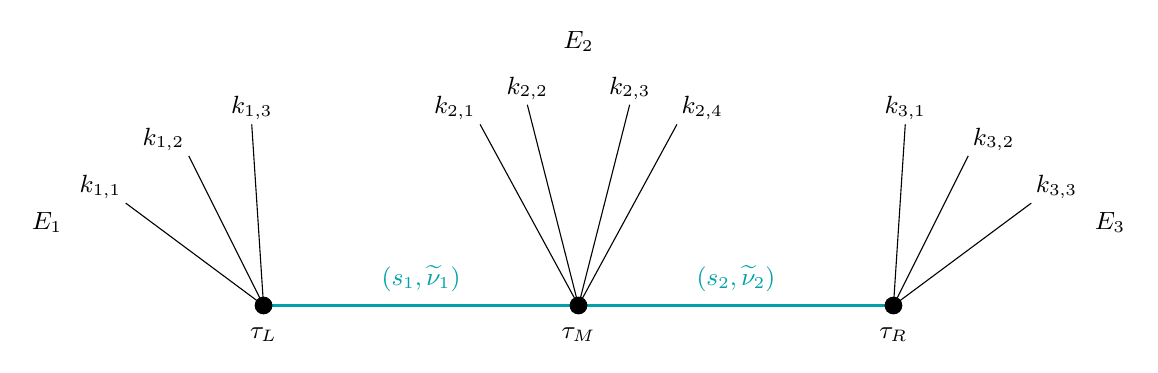
\begin{tikzpicture}[every node/.style={inner sep=1.5pt}]
  \coordinate (vL) at (0,0);
  \coordinate (vM) at (4.0,0);
  \coordinate (vR) at (8.0,0);
  % External-leg fans above each vertex; per-leg momentum labels at the tips,
  % summed energies E_v outside the fans.
  \draw (vL) -- (-1.75,1.30);
  \draw (vL) -- (-0.95,1.90);
  \draw (vL) -- (-0.15,2.30);
  \node[anchor=south east] at (-1.75,1.30) {\small $k_{1,1}$};
  \node[anchor=south east] at (-0.95,1.90) {\small $k_{1,2}$};
  \node[anchor=south]      at (-0.15,2.30) {\small $k_{1,3}$};
  \node at (-2.75,1.05) {\small $E_1$};
  \draw (vM) -- (2.75,2.30);
  \draw (vM) -- (3.35,2.55);
  \draw (vM) -- (4.65,2.55);
  \draw (vM) -- (5.25,2.30);
  \node[anchor=south east] at (2.75,2.30) {\small $k_{2,1}$};
  \node[anchor=south]      at (3.35,2.55) {\small $k_{2,2}$};
  \node[anchor=south]      at (4.65,2.55) {\small $k_{2,3}$};
  \node[anchor=south west] at (5.25,2.30) {\small $k_{2,4}$};
  \node at (4.0,3.35) {\small $E_2$};
  \draw (vR) -- (8.15,2.30);
  \draw (vR) -- (8.95,1.90);
  \draw (vR) -- (9.75,1.30);
  \node[anchor=south]      at (8.15,2.30) {\small $k_{3,1}$};
  \node[anchor=south west] at (8.95,1.90) {\small $k_{3,2}$};
  \node[anchor=south west] at (9.75,1.30) {\small $k_{3,3}$};
  \node at (10.75,1.05) {\small $E_3$};
  % Internal massive propagators: teal directed lines with parenthesised
  % (momentum, mass) labels above, arrows marking the momentum flow.
  \draw[->,thick,propblue] (vL) -- (vM);
  \draw[->,thick,propblue] (vM) -- (vR);
  \node[propblue] at (2.0,0.34) {\small $(s_1,\widetilde\nu_1)$};
  \node[propblue] at (6.0,0.34) {\small $(s_2,\widetilde\nu_2)$};
  % Vertex times below the vertices.
  \node[anchor=north] at (0,-0.22)   {\small $\tau_L$};
  \node[anchor=north] at (4.0,-0.22) {\small $\tau_M$};
  \node[anchor=north] at (8.0,-0.22) {\small $\tau_R$};
  % Vertices last.
  \filldraw[fill=black,draw=black] (vL) circle (3pt);
  \filldraw[fill=black,draw=black] (vM) circle (3pt);
  \filldraw[fill=black,draw=black] (vR) circle (3pt);
\end{tikzpicture}
\end{document}
